\documentclass[11pt]{article}

% ---------- Page geometry ----------
\usepackage[a4paper, margin=2.7cm]{geometry}

% ---------- Core packages ----------
\usepackage[T1]{fontenc}
\usepackage[utf8]{inputenc}
\usepackage{booktabs}
\usepackage{array}
\usepackage{amsmath}
\usepackage{siunitx}
\usepackage{graphicx}
\usepackage{xcolor}
\usepackage{tikz}
\usepackage{pgfplots}
\pgfplotsset{compat=1.18}
\usepackage{listings}
\usepackage{fancyhdr}
\usepackage{titlesec}
\usepackage{enumitem}
\usepackage[colorlinks=true, linkcolor=seaBlue, urlcolor=seaBlue, citecolor=seaBlue]{hyperref}

% ---------- Colors (consistent with the presentation) ----------
\definecolor{seaBlue}{RGB}{20,80,120}
\definecolor{seaTeal}{RGB}{30,140,140}
\definecolor{softGray}{RGB}{90,90,90}
\definecolor{noiseRed}{RGB}{200,60,50}
\definecolor{budgetGreen}{RGB}{60,150,80}

% ---------- Section heading style ----------
\titleformat{\section}{\normalfont\Large\bfseries\color{seaBlue}}{\thesection}{0.5em}{}
\titleformat{\subsection}{\normalfont\large\bfseries\color{seaTeal}}{\thesubsection}{0.5em}{}

% ---------- Header/footer ----------
\pagestyle{fancy}
\fancyhf{}
\fancyhead[L]{\small\textcolor{softGray}{Benchmarking FHE Libraries -- SEAL Results Report}}
\fancyhead[R]{\small\textcolor{softGray}{\thepage}}
\renewcommand{\headrulewidth}{0.4pt}

% ---------- Code listing style ----------
\lstset{
  basicstyle=\ttfamily\small,
  backgroundcolor=\color{black!4},
  frame=single,
  rulecolor=\color{black!20},
  breaklines=true,
  columns=fullflexible,
  keepspaces=true,
  showstringspaces=false,
}

% ---------- Helper commands ----------
\newcommand{\good}[1]{\textcolor{seaTeal}{\textbf{#1}}}

\begin{document}

% =====================================================================
% TITLE PAGE
% =====================================================================
\begin{titlepage}
  \centering
  \vspace*{0.8cm}

  % ---- Institution header (bilingual, matching reference structure exactly) ----
  \noindent
  \begin{minipage}[t]{0.46\textwidth}
  \centering\small\bfseries
  Universit\'e de Yaound\'e I\\[2pt]
  ********\\[2pt]
  \'Ecole Nationale Sup\'erieure Polytechnique\\[2pt]
  ********\\[2pt]
  D\'epartement de G\'enie informatique
  \end{minipage}
  \hfill
  \begin{minipage}[t]{0.46\textwidth}
  \centering\small\bfseries
  University of Yaounde I\\[2pt]
  ********\\[2pt]
  National Advanced School of Engineering of Yaounde\\[2pt]
  ********\\[2pt]
  Department of Computer Science
  \end{minipage}

  \vspace{0.7cm}

  % ---- Logos ----
  
\includegraphics[height=2.3cm]{logos/logo_uy1.jpeg}
  \hspace{1.4cm}
  
\includegraphics[height=2.3cm]{logos/logo_enspy.jpeg}

  \vspace{1.3cm}

  {\color{seaBlue}\rule{\linewidth}{1pt}}
  \vspace{0.5cm}

  {\huge\bfseries Benchmarking Fully Homomorphic\\[0.2cm] Encryption Libraries\par}
  \vspace{0.4cm}
  {\Large Results Report: Microsoft SEAL\par}

  \vspace{0.5cm}
  {\color{seaBlue}\rule{\linewidth}{1pt}}
  \vspace{1.6cm}

  \begin{minipage}{0.45\textwidth}
    \raggedright
    \textbf{Author}\\
    Boungo Tresor
  \end{minipage}
  \hfill
  \begin{minipage}{0.45\textwidth}
    \raggedleft
    \textbf{Supervisor}\\
    Dr.\ Herv\'e Tal\'e Kalachi
  \end{minipage}

  \vfill

  {\large \today\par}
  \vspace{0.5cm}
  {\small\textcolor{softGray}{Master's Thesis -- Progress Report}\par}

\end{titlepage}

\tableofcontents
\newpage

% =====================================================================
\section*{Abstract}
\addcontentsline{toc}{section}{Abstract}

This report presents the results obtained to date in a Master's thesis benchmarking Fully Homomorphic Encryption (FHE) libraries. The thesis compares library implementations of the BFV, BGV, and CKKS schemes across four libraries (Microsoft SEAL, OpenFHE, HElib, Lattigo) under a single, consistent evaluation framework. This report covers the first of these four libraries: \textbf{Microsoft SEAL}, evaluated across all three schemes, six metrics, and applicable scenarios, with documented scope limits at the largest ring dimension (Section~\ref{sec:limitations}).

Six metrics were measured -- latency, memory, energy, storage, noise-budget evolution, and CKKS error accumulation -- across three deployment scenarios (a full-resource baseline, a resource-constrained profile simulating a small edge device, and a batch/streaming profile) and a twelve-point parameter grid spanning four ring dimensions and three NIST-aligned security categories. This work's contribution is a unified, security-stratified evaluation that brings performance, energy-per-operation, memory/storage, and correctness/precision together under one consistent framework across FHE libraries.

Headline findings: SEAL's measured costs scale with ring dimension and security level as the underlying parameter tables predict; the Resource-Constrained x86 profile (4 cores / 4\,GB RAM cap) does not measurably affect performance at this workload scale; batching amortizes one-time key-generation cost but does not reduce the recurring cost of individual cryptographic operations; and noise-budget and CKKS-error tracking -- two independently implemented measurements -- agree on every parameter set tested, including the one configuration in the grid with no usable noise budget.

Section~\ref{sec:reproducibility} provides the complete information needed to reproduce every result in this report, including exact software versions, hardware specification, and a public code repository.

\vspace{0.3cm}
\noindent\textit{Remaining work: the same evaluation framework applied to OpenFHE, HElib, and Lattigo, followed by a cross-library comparison.}

\newpage

\section{Introduction and Scope}
\label{sec:intro}

This report covers progress on a Master's thesis benchmarking Fully Homomorphic Encryption (FHE) libraries -- Microsoft SEAL, OpenFHE, HElib, and Lattigo -- under one consistent methodology, so that results are directly comparable across libraries.

\textbf{Scope:} this report covers \textbf{Microsoft SEAL} (v4.1.2), the first of the four libraries: all six metrics (latency, memory, energy, storage, noise-budget evolution, CKKS error), across all applicable scenarios, over the full parameter grid at $N \le 8192$, extended to category~1 at $N=16384$. The remaining $N=16384$ cells were excluded on hardware-safety grounds (Section~\ref{sec:limitations}). OpenFHE, HElib, and Lattigo are ongoing work (Section~\ref{sec:nextsteps}).

Section~\ref{sec:reproducibility} gives everything needed to reproduce every result here independently: exact hardware, software versions, commands, and a public repository.

\section{Methodology}
\label{sec:methodology}

\subsection{Parameter space}

Every test is defined by four parameters, fixed before any measurement: ring dimension $N$, a modulus chain (built from several primes, chosen deterministically for fast arithmetic -- not random), the resulting multiplicative depth, and a security category mapped to NIST-aligned tiers (128/192/256-bit)~\cite{nist-pqc}. Table~\ref{tab:paramgrid} gives the full grid, verified against the Homomorphic Encryption Standard~\cite{hestandard2021,bossuat2024}.

\begin{table}[h!]
\centering\small
\begin{tabular}{@{}cccccc@{}}
\toprule
$N$ & Category & Max $\log q$ & Chain (bits) & $\log q$ used & Depth \\
\midrule
2048  & 1 (128-bit) & 54  & \{26,26\}             & 52  & 0 \\
2048  & 3 (192-bit) & 37  & \{17,17\}             & 34  & 0 \\
2048  & 5 (256-bit) & 29  & \{26\}                & 26  & 0 \\
4096  & 1 (128-bit) & 109 & \{33,33,34\}          & 100 & 1 \\
4096  & 3 (192-bit) & 75  & \{34,34\}             & 68  & 0 \\
4096  & 5 (256-bit) & 58  & \{27,28\}             & 55  & 0 \\
8192  & 1 (128-bit) & 218 & \{60,40,40,60\}       & 200 & 2 \\
8192  & 3 (192-bit) & 152 & \{46,47,47\}          & 140 & 1 \\
8192  & 5 (256-bit) & 118 & \{54,54\}             & 108 & 0 \\
16384 & 1 (128-bit) & 438 & \{60,40$\times$7,60\} & 400 & 7 \\
16384 & 3 (192-bit) & 305 & \{60,40$\times$4,60\} & 280 & 4 \\
16384 & 5 (256-bit) & 237 & \{60,40$\times$2,60\} & 200 & 2 \\
\bottomrule
\end{tabular}
\caption{Full parameter grid. Depth grows with $N$ and shrinks as the security requirement rises at fixed $N$ -- the same modulus that sets the noise budget also governs hardness, so a harder security target forces a smaller budget. Eight cells' chains were re-tuned from their original values (Section~\ref{sec:security-validation}) to meet the 2024/2025 guideline; $N{=}2048$/category~5's chain shrank to a single prime, the only cell in this grid with no dedicated key-switching modulus.}
\label{tab:paramgrid}
\end{table}

Each configuration was tested for all three of SEAL's supported schemes: BFV (exact arithmetic), BGV (exact arithmetic, alternative encoding), and CKKS (approximate arithmetic).

\subsection{Security-level validation}
\label{sec:security-validation}

The category labels in Table~\ref{tab:paramgrid} (128/192/256-bit) originate from the 2018 Homomorphic Encryption Standard's reference table. Since cryptanalysis has advanced since then, security was independently re-verified using the Lattice Estimator~\cite{albrecht2015estimator} (commit \texttt{3e48ef4}), against SEAL's actual distributions -- a uniform ternary secret and a Centered Binomial error distribution with $\sigma \approx 3.2$ (SEAL's compiled default; \texttt{SEAL\_USE\_GAUSSIAN\_NOISE} is not set in this build) -- rather than assumed generic parameters.

The verification proceeded in two stages. First, every configuration's $\log q$ (Table~\ref{tab:paramgrid}) was compared against the threshold in Table~\ref{tab:guideline52} -- an excerpt of Table 5.2 from the 2024/2025 Security Guidelines~\cite{bossuat2024}, reproduced here for the ring dimensions used in this thesis, itself built from the same estimator. Second, this comparison was validated directly: nine of the twelve configurations -- every configuration at $N \le 8192$ -- were also run through the estimator's own full \texttt{LWE.estimate()} routine, which evaluates every supported attack (uSVP, BDD, dual, dual-hybrid, coded-BKW) and reports the cheapest, and the results agreed closely with the guideline-based prediction in every case. A full run at $N=16384$ is highly resource-intensive, however -- a single run at $N=8192$ already took over two hours even with 12-way parallelism, and the tool's own issue tracker documents impractical runtimes above $N=2^{13}$ as a known limitation -- so the three $N=16384$ configurations were assessed from the guideline comparison alone.

\begin{table}[h!]
\centering\small
\begin{tabular}{@{}cccc@{}}
\toprule
$N$ & 128-bit & 192-bit & 256-bit \\
\midrule
2048  & 53  & 36  & 27 \\
4096  & 106 & 73  & 56 \\
8192  & 214 & 147 & 114 \\
16384 & 430 & 297 & 230 \\
\bottomrule
\end{tabular}
\caption{Maximum $\log q$ for each target level, uniform ternary secret, $\sigma{=}3.19$ Gaussian error -- excerpted from Table 5.2 of the 2024/2025 Security Guidelines~\cite{bossuat2024}, rows matching this thesis's ring dimensions only.}
\label{tab:guideline52}
\end{table}

Table~\ref{tab:secvalidation} gives the result for every configuration.

\begin{table}[h!]
\centering\small
\begin{tabular}{@{}cccp{5.2cm}@{}}
\toprule
$N$ & Category & Estimated security & Method \\
\midrule
2048  & 1 & 131.3 bits & Lattice Estimator \\
2048  & 3 & 205.3 bits & Lattice Estimator \\
2048  & 5 & 272.0 bits & Lattice Estimator \\
4096  & 1 & 137.2 bits & Lattice Estimator \\
4096  & 3 & 208.6 bits & Lattice Estimator \\
4096  & 5 & 263.3 bits & Lattice Estimator \\
8192  & 1 & 137.7 bits & Lattice Estimator \\
8192  & 3 & 204.1 bits & Lattice Estimator \\
8192  & 5 & 272.8 bits & Lattice Estimator \\
16384 & 1 & $\geq$128 bits ($\log q$ under threshold by 30 bits) & Guideline Table 5.2 \\
16384 & 3 & $\geq$192 bits ($\log q$ under threshold by 17 bits) & Guideline Table 5.2 \\
16384 & 5 & $\geq$256 bits ($\log q$ under threshold by 30 bits) & Guideline Table 5.2 \\
\bottomrule
\end{tabular}
\caption{Estimated real security per configuration. Category numbers refer to the NIST-aligned tiers defined in Table~\ref{tab:paramgrid}. All values represent an infeasible amount of computation for an attacker regardless of method.}
\label{tab:secvalidation}
\end{table}

Every configuration in Table~\ref{tab:secvalidation} requires well over $2^{120}$ operations to attack -- far beyond any practically exploitable threshold under any of the methods used. Estimated security is now tightest at $N{=}2048$, category~1 (131.3 bits, only 3.3 bits above its 128-bit target) -- the direct cost of the correctness-driven trade-off discussed below, where this cell's chain could not be shrunk much further below the guideline threshold without losing noise budget entirely. Category~5 configurations retain the widest margins across all three ring dimensions (16+ bits above their 256-bit target at $N{=}2048$ and $N{=}8192$), since their much smaller absolute $\log q$ budgets left more room to land comfortably under the 2024/2025 guideline ceiling once re-tuned.

Shrinking three of these chains for security compliance left too little coefficient-modulus budget to survive even a single homomorphic operation under BFV/BGV's standard plaintext modulus (SEAL's 20-bit batching prime, $t=1032193$, used by every other cell in this grid): fresh ciphertexts at these three configurations decrypted with zero remaining noise budget regardless of the operation performed. Each was instead given the smallest batching-compatible plaintext modulus that restored a real, positive noise-budget margin after the cell's actual required operation (Table~\ref{tab:configmeta-bfvbgv}).

\begin{table}[h!]
\centering\small
\begin{tabular}{@{}ccll@{}}
\toprule
$N$ & Category & Plaintext modulus $t$ & Noise budget margin after real op \\
\midrule
2048 & 1 & 12289 (14-bit) & 5 bits (after add) \\
2048 & 5 & 12289 (14-bit) & 1 bit (after add) \\
4096 & 5 & 40961 (16-bit) & 4 bits (after add) \\
\bottomrule
\end{tabular}
\caption{The three cells using a plaintext modulus other than this grid's standard $t=1032193$ (20-bit SEAL batching prime), and the resulting noise-budget margin after the cell's real required operation (add, since all three are depth-0). Necessary because their reduced coeff-modulus chains (Table~\ref{tab:paramgrid}) leave zero noise budget under the standard $t$ -- fresh ciphertexts otherwise fail to decrypt correctly at all. Every other BFV/BGV cell in the grid is unaffected and keeps $t=1032193$.}
\label{tab:configmeta-bfvbgv}
\end{table}

$N{=}2048$/category~5's 1-bit margin is the thinnest in the grid. Before being accepted into the main results, it was stability-tested separately with 50 independent trials -- fresh random data each trial, encrypt $\to$ add $\to$ decrypt $\to$ decode against the exact expected result -- and all 50 decoded correctly.

The same reduced chains created an analogous problem for CKKS's initial scale. This project's default formula (min(40, $(\text{total\_bits}-10)/2$) bits, reserving headroom for one future multiply) gave unusably imprecise results at four of the affected depth-0 cells -- that reserved multiply headroom is precision they never spend, since they never multiply -- and left one comfortably-working cell more conservative than it needed to be. Each was given the empirically best scale found by direct round-trip testing against its new chain (Table~\ref{tab:configmeta-ckks}); the two affected depth-1 cells ($N{=}4096$/category~1 and $N{=}8192$/category~3) already worked well under the default formula and were left unchanged.

\begin{table}[h!]
\centering\small
\begin{tabular}{@{}cclp{4.5cm}@{}}
\toprule
$N$ & Category & Scale & Resulting error (max / mean) \\
\midrule
2048 & 1 & $2^{24}$ & $1.8{\times}10^{-4}$ / $2.0{\times}10^{-5}$ -- usable \\
2048 & 3 & $2^{15}$ & $0.08$ / $0.01$ -- best achievable at this $N$/chain, not a clean fix (see note below) \\
4096 & 3 & $2^{32}$ & $1.1{\times}10^{-6}$ / $1.7{\times}10^{-7}$ -- good \\
4096 & 5 & $2^{24}$ & $2.9{\times}10^{-4}$ / $4.2{\times}10^{-5}$ -- good \\
8192 & 5 & $2^{40}$ & $1.1{\times}10^{-8}$ / $1.3{\times}10^{-9}$ -- comfortable \\
\bottomrule
\end{tabular}
\caption{The five CKKS cells using a scale other than the default formula's output. $N{=}8192$/category~5's default formula would have given $2^{24}$ (borderline, max error $7.3{\times}10^{-4}$); $2^{40}$ was adopted instead since it is strictly better and brings this cell in line with every other comfortably-precise cell, not because the default was broken. Every other CKKS cell in the grid is unaffected. Error figures are decoded-vs-exact absolute error over uniform-random $[-1,1]$ input, mirroring the ckks\_error trace's own methodology (fresh $\to$ add for depth-0 cells; fresh $\to$ add $\to$ multiply $\to$ relinearize $\to$ rescale for depth-1 cells).}
\label{tab:configmeta-ckks}
\end{table}

$N{=}2048$/category~3 is a genuine structural limitation, not a tuning gap: at this chain's total coefficient-modulus budget of only 17 bits, $2^{15}$ is one bit below the point where SEAL itself refuses the scale as out of bounds, and even at that ceiling roughly 8\% max decode error remains. This mirrors $N{=}2048$/category~5's single-prime BFV chain (Section~\ref{sec:security-validation}) -- both are cases where the security fix leaves too little raw budget for this scheme to represent values comfortably, independent of how carefully the remaining parameter is tuned. Wherever this cell's CKKS results appear, they should carry that caveat and not be presented as directly comparable to the grid's other CKKS cells.

\subsection{Metrics}

Six metrics were measured (Table~\ref{tab:metrics}). Rather than resting on any single metric being unprecedented, this work's contribution is the combination: a unified, security-stratified evaluation bringing performance, energy-per-operation, memory/storage, and correctness/precision together under one consistent framework.

\begin{table}[h!]
\centering\small
\begin{tabular}{@{}llp{5.3cm}@{}}
\toprule
\textbf{Metric} & \textbf{Precedent} & \textbf{Description} \\
\midrule
Latency & standard in prior work & Time per operation \\
Memory & standard in prior work & Peak RAM used \\
Energy & none found in papers surveyed & Electrical energy per operation (RAPL) \\
Storage & Pambudi et al.~\cite{pambudi2025} & Serialized ciphertext/key size \\
Noise budget & Pambudi et al.~\cite{pambudi2025} & Remaining margin before decryption fails \\
CKKS error & Takeshita et al.~\cite{takeshita2025} & Drift from the exact result \\
\bottomrule
\end{tabular}
\caption{Metrics measured, with literature precedent.}
\label{tab:metrics}
\end{table}

\subsection{Deployment scenarios}

Latency, memory, and energy were measured under three scenarios (Table~\ref{tab:scenarios}). Storage, noise budget, and CKKS error depend only on the parameters, not on machine resources or request volume, so each was measured once across the full grid.

\begin{table}[h!]
\centering\small
\begin{tabular}{@{}lll@{}}
\toprule
\textbf{Scenario} & \textbf{Configuration} & \textbf{Question answered} \\
\midrule
Standard & Full workstation resources & Baseline cost \\
Constrained & 4 cores / 4\,GB RAM cap~\cite{rahman2024} & Sensitivity to limited resources \\
Edge/Batch & Batch sizes 1/10/100~\cite{gouert2023} & Behavior under continuous load \\
\bottomrule
\end{tabular}
\caption{Deployment scenarios.}
\label{tab:scenarios}
\end{table}

Coverage differs by scenario at the largest ring dimension. The Standard scenario was run across the full grid at $N \in \{2048, 4096, 8192\}$ and extended to $N=16384$ for category~1; categories 3 and 5 at $N=16384$ for the Standard scenario, and $N=16384$ entirely for the Constrained and Edge/Batch scenarios and the parameter-only storage, noise-budget, and CKKS-error measurements, were excluded from this evaluation and run only up to $N=8192$. This is a deliberate scope decision made after sustained runs at $N=16384$ produced thermal instability on the development workstation (Section~\ref{sec:limitations}), not a gap left unacknowledged; any incomplete cells within the reported scope are flagged rather than omitted in the results tables of Section~\ref{sec:results}.

\subsection{Statistical protocol}

Each timed operation ran 105 times; the first 5 were discarded as cache warm-up, leaving 100 runs per reported value. Results are reported as mean, standard deviation, and 95\% confidence interval. Results with standard deviation exceeding 5\% of the mean are flagged \texttt{HIGH\_VARIANCE} rather than hidden.

\subsection{Tool validation}

Three different validation methods were used, matched to what each tool measures. Timing and correctness tools were checked by reproducing a prior published benchmark (HEProfiler) under identical parameters. The energy tool (Intel's RAPL hardware counters) has no prior FHE benchmark to reproduce against, so it instead relies on RAPL's own accuracy literature~\cite{khan2018}. Security-level mapping is validated against the published Homomorphic Encryption Standard and its 2024 update~\cite{hestandard2021,bossuat2024}, the same reference the parameter grid itself is built from.

\section{Results}
\label{sec:results}

This section presents the results obtained for SEAL. Latency figures are drawn from the Standard scenario; storage, noise budget, and CKKS error are properties of the parameters themselves and were measured once across the full grid (Section~\ref{sec:methodology}).

\subsection{Latency}

Table~\ref{tab:latency} gives the range of each operation's cost across every tested parameter combination. 83 of 112 latency measurements were flagged \texttt{HIGH\_VARIANCE} -- expected for fast operations, where ordinary background noise is large relative to the operation itself.

\begin{table}[h!]
\centering\small
\begin{tabular}{@{}lccl@{}}
\toprule
\textbf{Operation} & \textbf{Min (ms)} & \textbf{Max (ms)} & \textbf{Comment} \\
\midrule
add & 0.005 & 0.52 & negligible cost \\
decrypt & 0.01 & 4.22 & fast \\
encrypt & 0.35 & 12.90 & moderate \\
relinearize & 0.58 & 18.93 & moderate \\
multiply & 0.16 & 49.18 & slowest single operation \\
keygen & 14.48 & 277.89 & slowest overall -- but runs once \\
\bottomrule
\end{tabular}
\caption{Latency range across the full parameter grid, Standard scenario.}
\label{tab:latency}
\end{table}

\begin{figure}[h!]
\centering
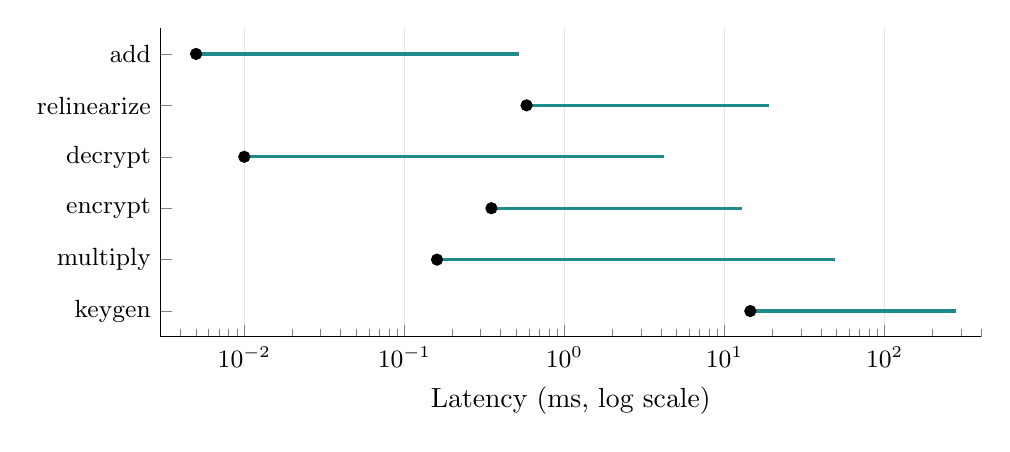
\begin{tikzpicture}
  \begin{axis}[
      width=12cm, height=5.5cm,
      xmode=log,
      xlabel={Latency (ms, log scale)},
      symbolic y coords={add,relinearize,decrypt,encrypt,multiply,keygen},
      ytick=data, y dir=reverse,
      xmin=0.003, xmax=400,
      axis lines*=left,
      xmajorgrids, grid style={gray!20},
      tick label style={font=\small},
    ]
    \addplot[only marks, mark=none, forget plot] coordinates
      {(0.005,add) (0.58,relinearize) (0.01,decrypt) (0.35,encrypt) (0.16,multiply) (14.5,keygen)};
    \draw[very thick, seaTeal] (axis cs:0.005,add) -- (axis cs:0.52,add);
    \draw[very thick, seaTeal] (axis cs:0.58,relinearize) -- (axis cs:19,relinearize);
    \draw[very thick, seaTeal] (axis cs:0.01,decrypt) -- (axis cs:4.2,decrypt);
    \draw[very thick, seaTeal] (axis cs:0.35,encrypt) -- (axis cs:12.9,encrypt);
    \draw[very thick, seaTeal] (axis cs:0.16,multiply) -- (axis cs:49,multiply);
    \draw[very thick, seaTeal] (axis cs:14.5,keygen) -- (axis cs:278,keygen);
  \end{axis}
\end{tikzpicture}
\caption{Latency range per operation, Standard scenario, log scale. Each bar spans every tested parameter combination.}
\label{fig:latency}
\end{figure}

Every operation is fast in absolute terms; the real difference is relative -- multiply and keygen cost 10--100$\times$ more than add or decrypt.

\clearpage
\subsection{Storage, noise budget, and CKKS error}

\subsubsection*{Storage}

Table~\ref{tab:storage} and Figure~\ref{fig:storage} give serialized sizes for all four artifact types at two ring dimensions.

\begin{table}[h!]
\centering\small
\begin{tabular}{@{}lcccc@{}}
\toprule
& \textbf{Ciphertext} & \textbf{Public key} & \textbf{Secret key} & \textbf{Relin.\ keys} \\
\midrule
$N{=}8192$ (MB) & 0.39 & 0.52 & 0.26 & 1.57 \\
$N{=}16384$ (MB) & 2.10 & 2.36 & 1.18 & 18.88 \\
\bottomrule
\end{tabular}
\caption{Serialized artifact sizes, category 1 (128-bit).}
\label{tab:storage}
\end{table}

\begin{figure}[h!]
\centering
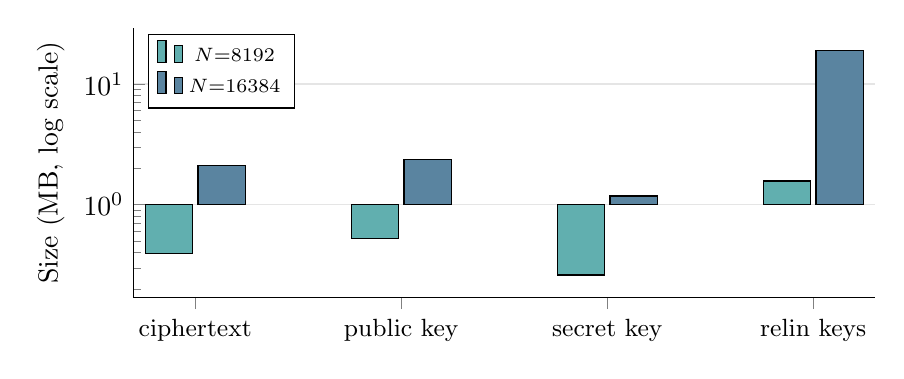
\begin{tikzpicture}
  \begin{axis}[
      width=11cm, height=5cm,
      ybar, bar width=0.6cm,
      ymode=log,
      symbolic x coords={ciphertext, public key, secret key, relin keys},
      xtick=data, x tick label style={font=\small},
      ylabel={Size (MB, log scale)},
      legend style={font=\scriptsize, at={(0.02,0.98)}, anchor=north west},
      axis lines*=left,
      ymajorgrids, grid style={gray!20},
    ]
    \addplot[fill=seaTeal!70] coordinates {(ciphertext,0.393) (public key,0.524) (secret key,0.262) (relin keys,1.573)};
    \addplot[fill=seaBlue!70] coordinates {(ciphertext,2.097) (public key,2.359) (secret key,1.180) (relin keys,18.875)};
    \legend{$N{=}8192$, $N{=}16384$}
  \end{axis}
\end{tikzpicture}
\caption{Serialized storage by artifact type and ring dimension (log scale).}
\label{fig:storage}
\end{figure}

The relinearization key is consistently the largest artifact -- roughly $12\times$ the ciphertext size at $N{=}16384$.

The Composite scenario's Galois (rotation) keys are a more extreme case, and one this harness got wrong until an extra-rigor correctness pass caught it: SEAL's \texttt{create\_galois\_keys()} generates a key for every power-of-two rotation step the scheme supports by default, not just the step(s) a given operation actually rotates by. A single rotate-by-1 measurement ($N{=}8192$, category~1) originally generated a 36.07\,MB key this way; requesting only the specific step actually used (via the explicit-steps overload) reduces this to 1.56\,MB -- a 23$\times$ reduction, with no change to correctness (verified by direct measurement, not assumed).

\subsubsection*{Noise budget}

Figure~\ref{fig:noisebudget} plots two complete, real traces: the shallowest usable depth (depth 2) and the deepest tested (depth 7, $N{=}16384$). Both stay well above zero through their full documented chain.

\begin{figure}[h!]
\centering
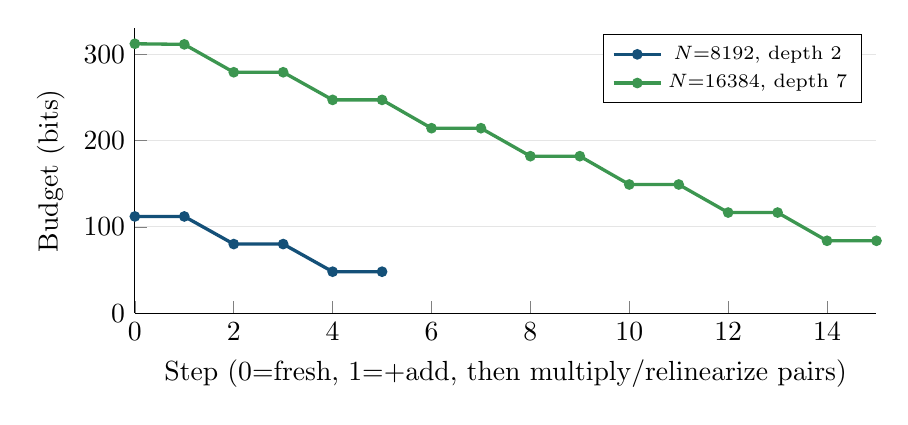
\begin{tikzpicture}
  \begin{axis}[
      width=11cm, height=5.2cm,
      xlabel={Step (0=fresh, 1=+add, then multiply/relinearize pairs)},
      ylabel={Budget (bits)},
      xmin=0, xmax=15, ymin=0, ymax=330,
      axis lines*=left,
      ymajorgrids, grid style={gray!20},
      legend style={font=\scriptsize, at={(0.98,0.98)}, anchor=north east},
    ]
    \addplot[very thick, mark=*, mark size=1.3pt, seaBlue] coordinates
      {(0,112)(1,112)(2,80)(3,80)(4,48)(5,48)};
    \addplot[very thick, mark=*, mark size=1.3pt, budgetGreen] coordinates
      {(0,312)(1,311.3)(2,279)(3,279)(4,247)(5,247)(6,214.2)(7,214.2)(8,181.8)(9,181.8)
       (10,149)(11,149)(12,116.5)(13,116.5)(14,83.8)(15,83.8)};
    \legend{{$N{=}8192$, depth 2}, {$N{=}16384$, depth 7}}
  \end{axis}
\end{tikzpicture}
\caption{Noise-budget evolution, both real, complete traces.}
\label{fig:noisebudget}
\end{figure}

The one exception in the whole grid: $N{=}2048$, category~1 -- budget is \textbf{0} already on the fresh ciphertext, before any operation runs (Table~\ref{tab:zerobudget}).

Three configurations in this grid -- $N{=}2048$/category~1, $N{=}2048$/category~5, and $N{=}4096$/category~5 -- use a smaller plaintext modulus than the rest (Section~\ref{sec:security-validation}, Table~\ref{tab:configmeta-bfvbgv}), so their noise-budget numbers are not directly comparable to the other nine configurations' on that basis alone.

\begin{table}[h!]
\centering\small
\begin{tabular}{@{}lcc@{}}
\toprule
& \textbf{Fresh} & \textbf{After +add} \\
\midrule
$N{=}2048$, category 1 & 0 bits & 0 bits \\
$N{=}2048$, category 3 & 6 bits & 5.9 bits \\
\bottomrule
\end{tabular}
\caption{Noise budget at the smallest ring dimension.}
\label{tab:zerobudget}
\end{table}

\subsubsection*{CKKS error}

Figure~\ref{fig:ckkserror} compares the grid's two thinnest-budget configurations -- $N{=}2048$/category~1 (zero budget, Table~\ref{tab:zerobudget}) and $N{=}2048$/category~3 (6 bits, non-zero but thin) -- against two comfortably-budgeted configurations, all measured at the same step (after the first addition) for a fair comparison.

\begin{figure}[h!]
\centering
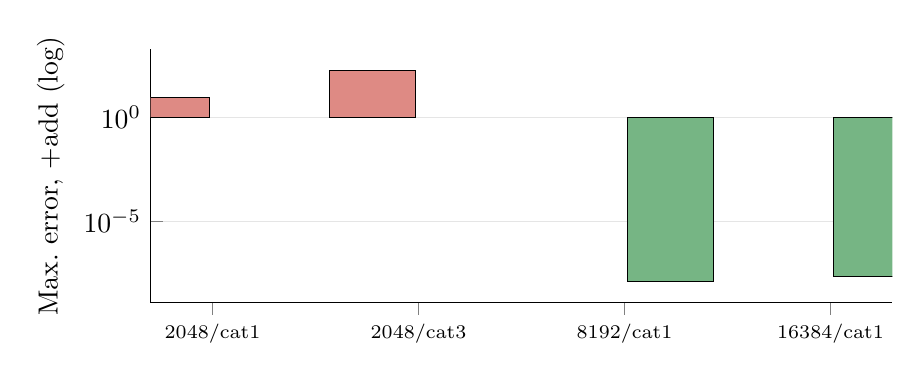
\begin{tikzpicture}
  \begin{axis}[
      width=11cm, height=4.8cm,
      ybar, bar width=1.1cm,
      symbolic x coords={A, B, C, D},
      xtick={A, B, C, D},
      x tick label style={font=\scriptsize, align=center},
      xticklabels={2048/cat1, 2048/cat3, 8192/cat1, 16384/cat1},
      ymode=log,
      ylabel={Max.\ error, +add (log)},
      axis lines*=left,
      ymajorgrids, grid style={gray!20},
    ]
    \addplot[fill=noiseRed!60] coordinates {(A,9.34) (B,176.2)};
    \addplot[fill=budgetGreen!70] coordinates {(C,1.31e-8) (D,2.30e-8)};
  \end{axis}
\end{tikzpicture}
\caption{CKKS error: zero- and thin-budget configurations vs.\ comfortably-budgeted ones (log scale).}
\label{fig:ckkserror}
\end{figure}

Both the zero-budget and the thin-budget configuration show error of order 1--100 -- unusable; notably, even a non-zero 6-bit budget is not enough to keep CKKS error under control. The two comfortably-budgeted configurations stay near $10^{-8}$, even at depth $>0$. Two independently implemented measurements -- noise-budget tracking (BFV, counts bits) and CKKS error tracking (diffs decrypted output against exact arithmetic) -- agree at every parameter set tested, including the one configuration with truly zero budget. This agreement is strong evidence the finding reflects the underlying parameters, not a measurement artifact.

\clearpage
\subsection{Behavior under different conditions}

\subsubsection*{Resource constraints}

SEAL's peak memory use (118.66\,MB, Standard; 118.77\,MB, Constrained) stays under 3\% of the 4\,GB Constrained-scenario cap. Standard and Constrained produced the same 112 succeeded / 24 skipped / 8 failed pattern, and latency ranges were statistically indistinguishable between the two (Table~\ref{tab:constrained}).

\begin{table}[h!]
\centering\small
\begin{tabular}{@{}lcc@{}}
\toprule
& \textbf{Standard} & \textbf{Constrained} \\
\midrule
Peak memory (max, MB) & 118.66 & 118.77 \\
Energy per op (max, J) & 7.42 & 5.39 \\
\texttt{HIGH\_VARIANCE} count & 83/112 & 63/112 \\
\bottomrule
\end{tabular}
\caption{Standard vs.\ Constrained, full grid.}
\label{tab:constrained}
\end{table}

The lower variance count under Constrained is consistent with core-pinning reducing scheduling noise, on top of the resource cap itself never binding at this workload scale.

\subsubsection*{Batching}

Figure~\ref{fig:batching} shows key-generation cost amortizing cleanly with batch size; every other operation showed no consistent change (ratios 0.82$\times$--1.49$\times$, no direction) -- each item was already at its most SIMD-efficient shape from the first ciphertext.

\begin{figure}[h!]
\centering
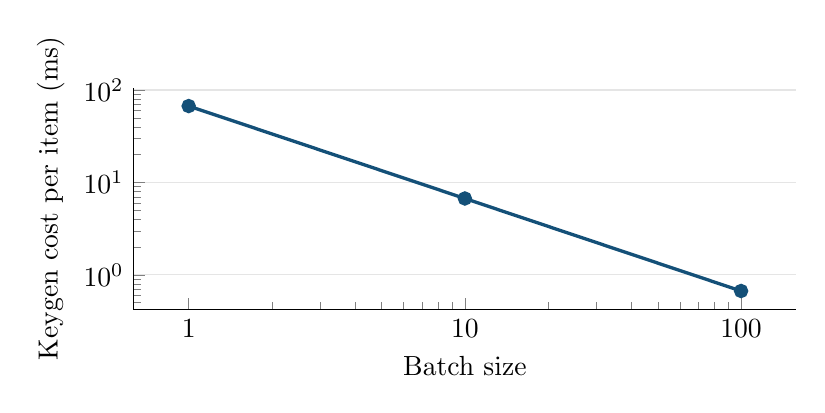
\begin{tikzpicture}
  \begin{axis}[
      width=10cm, height=4.4cm,
      xmode=log, ymode=log,
      xlabel={Batch size}, ylabel={Keygen cost per item (ms)},
      xtick={1,10,100}, xticklabels={1,10,100},
      axis lines*=left,
      ymajorgrids, grid style={gray!20},
    ]
    \addplot[very thick, mark=*, seaBlue] coordinates {(1,67.10) (10,6.71) (100,0.67)};
  \end{axis}
\end{tikzpicture}
\caption{Key-generation cost per item vs.\ batch size, $N{=}8192$/category~1 (log--log).}
\label{fig:batching}
\end{figure}

\textbf{Practical implication:} generate keys once and reuse them across every future operation; batching requests together does not reduce the cost of the underlying cryptographic operations.

\section{Limitations}
\label{sec:limitations}

Stated plainly rather than left implicit:

\begin{itemize}[leftmargin=*, itemsep=2pt]
  \item \textbf{$N{=}2048$, category 5} fails to build entirely -- SEAL's prime search cannot find enough NTT-friendly primes at this combination of ring size and security level. This is a genuine library limitation, not a bug; it is documented, not patched around.
  \item \textbf{Energy is not isolated to the benchmark process.} RAPL measures total package power draw during the measurement window, not one process's share of it. Background load was minimized but not eliminated.
  \item \textbf{No DRAM-domain energy is available on this hardware.} Only \texttt{package-0} and a \texttt{core} subzone are exposed under \texttt{/sys/class/powercap/}; package energy is the value reported throughout this report.
  \item \textbf{Apparent per-item energy improvement at larger batch sizes} (Section~\ref{sec:results}) is attributed to fixed Docker invocation overhead amortizing over more work, not a genuine drop in per-operation energy cost -- consistent with the flat per-item latency result.
  \item \textbf{The Constrained (``Resource-Constrained x86'') scenario reproduces a resource ceiling, not an architecture.} No physical ARM device was available; the 4-core/4\,GB cap was applied to the same x86-64 workstation via Docker, with the specific cap values drawn from Rahman et al.~\cite{rahman2024}'s Raspberry Pi 4 profile. This tests sensitivity to limited resources, not genuine cross-architecture behavior.
  \item \textbf{Testing at $N=16384$ was limited to category~1 of the Standard scenario.} This is the largest and most resource-intensive configuration in the grid; sustained multi-hour runs at this size produced thermal instability on the development workstation, including an unrelated display fault that required investigation before testing could safely resume. On these safety grounds, categories 3 and 5 at $N=16384$ for the Standard scenario, and $N=16384$ entirely for the Constrained, Edge/Batch, and parameter-only (storage, noise budget, CKKS error) measurements, were excluded from this evaluation and instead run only up to $N=8192$.
\end{itemize}

\section{Reproducibility}
\label{sec:reproducibility}

Everything needed to reproduce every result in this report is given below.

\subsection{Environment}

\begin{table}[h!]
\centering\small
\begin{tabular}{@{}ll@{}}
\toprule
\textbf{Component} & \textbf{Version / specification} \\
\midrule
CPU & AMD Ryzen 9 6900HX with Radeon Graphics \\
RAM & 14\,GiB \\
OS & Ubuntu 24.04.4 LTS (noble) \\
Kernel & Linux 7.0.0-28-generic, x86\_64 \\
Docker & 29.7.1 (build e9452d6) \\
g++ & 13.3.0 (Ubuntu 13.3.0-6ubuntu2\textasciitilde24.04.1) \\
CMake & 3.28.3 \\
SEAL & 4.1.2, Release, ZLIB/ZSTD on, HEXL off, Blake2xb PRNG \\
\bottomrule
\end{tabular}
\caption{Exact hardware and software environment.}
\label{tab:env}
\end{table}

\noindent\textit{Note:} energy is read from \texttt{/sys/class/powercap/intel-rapl:0/energy\_uj} (the \texttt{package-0} domain), in microjoules. This path is served by the \texttt{intel\_rapl\_msr} and \texttt{intel\_rapl\_common} kernel drivers -- confirmed via \texttt{lsmod} and the kernel boot log -- not the separate \texttt{amd\_energy} hwmon driver; AMD's RAPL-compatible model-specific registers are read through the same driver Intel systems use, which is also why the sysfs path keeps the \texttt{intel-rapl} name on this AMD CPU. The underlying hardware resolution is $2^{-16}$\,J $\approx 15.26\,\mu$J per step (from the kernel boot log), and the counter updates continuously rather than on a fixed polling interval, confirmed by rapid back-to-back reads showing a fresh value almost every time. The counter wraps at \texttt{max\_energy\_range\_uj} $=$ 65{,}532{,}610{,}987\,$\mu$J ($\approx$65.5\,kJ, roughly 14--24 minutes of continuous runtime depending on load); \texttt{run\_standard\_docker.sh} already accounts for this, detecting \texttt{E\_AFTER} $<$ \texttt{E\_BEFORE} and adding the range back before computing the delta.

\subsection{Code and data}

Source code, build scripts, and configuration are version-controlled at:
\begin{center}
\url{https://github.com/KingT1123/fhe-benchmark-suite}
\end{center}
Result data is deliberately \emph{not} version-controlled -- it is regenerated output, not source. The full parameter grid (Table~\ref{tab:paramgrid}) is at \texttt{experiments/config/param\_grid.csv}. Random inputs use a fixed seed, so repeated runs are reproducible; small numeric variation between runs (captured by the confidence intervals reported throughout) is expected from ordinary system timing noise, not from the random inputs themselves.

\subsection{Reproduction steps}

\begin{lstlisting}
git clone https://github.com/KingT1123/fhe-benchmark-suite.git
cd fhe-benchmark-suite/experiments/seal

# 1. Build the SEAL Docker image and compile the harness
bash docker_build_and_run.sh

# 2. Run each scenario (from experiments/scripts/)
cd ../scripts
bash run_standard_docker.sh
bash run_constrained_docker.sh
bash run_edge_batch_docker.sh
# storage, noise budget, CKKS error:
bash run_extended_metrics_docker.sh

# 3. Aggregate raw output into final results
python3 aggregate.py --scenario=standard
python3 aggregate.py --scenario=constrained
python3 aggregate.py --scenario=edge_batch
python3 aggregate.py --scenario=size
python3 aggregate.py --scenario=noise_trace
python3 aggregate.py --scenario=ckks_error
\end{lstlisting}

Energy measurement requires \texttt{sudo} for RAPL access; the run scripts prompt for this where needed.

\subsection{Output layout}

\begin{center}
\small
\begin{tabular}{@{}lp{8.5cm}@{}}
\toprule
\textbf{Path} & \textbf{Contents} \\
\midrule
\texttt{experiments/results/raw/} & Per-configuration raw output, Standard/Constrained \\
\texttt{experiments/results/raw/edge\_batch/} & Raw output, Edge/Batch scenario \\
\texttt{experiments/results/raw/extended\_metrics/} & Raw storage/noise/CKKS-error output \\
\texttt{experiments/results/final/} & Aggregated CSVs -- the source for every table and figure in this report \\
\bottomrule
\end{tabular}
\end{center}

\section{Next Steps}
\label{sec:nextsteps}

SEAL is now fully closed out against every metric and scenario defined in Section~\ref{sec:methodology}. The same framework -- unchanged parameter grid, unchanged metrics, unchanged statistical protocol -- will be applied next to \textbf{OpenFHE}, then \textbf{HElib} and \textbf{Lattigo}. OpenFHE supports a third scheme (BGV, in addition to BFV and CKKS); the other two dimensions of the methodology carry over directly.

Once all four libraries are evaluated, the final deliverable is a direct cross-library comparison -- same scheme against same scheme, under identical conditions -- which no library's individual results, including SEAL's above, can substitute for on their own.

\newpage
\section*{References}
\addcontentsline{toc}{section}{References}
\begin{thebibliography}{99}
\small

\bibitem{gouert2023} C. Gouert, D. Mouris, N.\,G. Tsoutsos. SoK: New Insights into Fully Homomorphic Encryption Libraries via Standardized Benchmarks. \emph{Proceedings on Privacy Enhancing Technologies}, 2023(3), 154--172. \url{https://doi.org/10.56553/popets-2023-0075}

\bibitem{rahman2024} T. Rahman, A.\,M.\,I.\,M. Osmani, M.\,S. Rahman, M.\,M.\,A. Shibly, S. Islam. Benchmarking Fully Homomorphic Encryption Libraries in IoT Devices. In \emph{NSysS '24}, pp.\ 16--23, ACM, 2024. \url{https://doi.org/10.1145/3704522.3704546}

\bibitem{pambudi2025} D.\,S. Pambudi, H. Studiawan, B.\,A. Pratomo, D. Purwitasari. Performance Analysis of Leading Homomorphic Encryption Libraries: A Benchmark Study of SEAL, HElib, OpenFHE, and Lattigo. In \emph{CSAIDE '25}, pp.\ 25--30, ACM, 2025. \url{https://doi.org/10.1145/3729706.3729711}

\bibitem{takeshita2025} J. Takeshita, N. Koirala, C. McKechney, T. Jung. HEProfiler: An In-Depth Profiler of Approximate Homomorphic Encryption Libraries. \emph{Journal of Cryptographic Engineering}, 15(2), Article 14, 2025. \url{https://doi.org/10.1007/s13389-025-00377-5}

\bibitem{khan2018} K.\,N. Khan, M. Hirki, T. Niemi, J.\,K. Nurminen, Z. Ou. RAPL in Action: Experiences in Using RAPL for Power Measurements. \emph{ACM Transactions on Modeling and Performance Evaluation of Computing Systems}, 3(2), Article 9, 2018. \url{https://doi.org/10.1145/3177754}

\bibitem{desrochers2016} S. Desrochers, C. Paradis, V.\,M. Weaver. A Validation of DRAM RAPL Power Measurements. In \emph{MEMSYS '16}, pp.\ 455--470, ACM, 2016. \url{https://doi.org/10.1145/2989081.2989088}

\bibitem{hestandard2021} M. Albrecht, M. Chase, H. Chen, J. Ding, S. Goldwasser, S. Gorbunov, S. Halevi, J. Hoffstein, K. Laine, K. Lauter, et al. Homomorphic Encryption Standard. In \emph{Protecting Privacy through Homomorphic Encryption}, pp.\ 31--62, 2021. \url{http://homomorphicencryption.org/wp-content/uploads/2018/11/HomomorphicEncryptionStandardv1.1.pdf}

\bibitem{bossuat2024} J.-P. Bossuat, R. Cammarota, I. Chillotti, B.\,R. Curtis, W. Dai, H. Gong, E. Hales, D. Kim, B. Kumara, C. Lee, et al. Security Guidelines for Implementing Homomorphic Encryption. \emph{Cryptology ePrint Archive}, Paper 2024/463, 2024; formally published as \emph{IACR Communications in Cryptology}, 1(4), 2025. \url{https://eprint.iacr.org/2024/463}

\bibitem{albrecht2015estimator} M.\,R. Albrecht, R. Player, S. Scott. On the concrete hardness of Learning with Errors. \emph{Journal of Mathematical Cryptology}, 9(3), 169--203, 2015. Lattice Estimator implementation: \url{https://github.com/malb/lattice-estimator}, commit \texttt{3e48ef4}.

\bibitem{nist-pqc} National Institute of Standards and Technology (NIST). Post-Quantum Cryptography: Security (Evaluation Criteria). \emph{NIST Computer Security Resource Center}. \url{https://csrc.nist.gov/projects/post-quantum-cryptography}

\end{thebibliography}


\end{document}
